\subsection{Overview}
\begin{frame}
    
    \begin{itemize}
        \item Describe problems on high level
    \end{itemize}

\end{frame}

%%%%%%%%%%%%%%%%%%%%%%%%%%%%%%%%%%%%%%%%%%%%%%%%%%%%%%%%%%%%%%%%%%%%%%%%%%%%%%%%

\subsection{VERA Problem 4}
\begin{frame}[t]{Problem Description}
    
\begin{columns}
    \begin{column}{0.5\textwidth}
        \begin{itemize}
            \item Center 3x3 assembly cluster in Watts Bar Unit 1
            \item AIC control rod in center assembly placed at 257.9 cm
            \item Test cases used 57 planes, with rod inserted 50\% into a plane
            \item Reference used 58 planes, with extra plane boundary aligned 
            with rod tip
            \item All simulations used 1 core per plane
        \end{itemize}
    \end{column}
    \begin{column}{0.28\textwidth}
        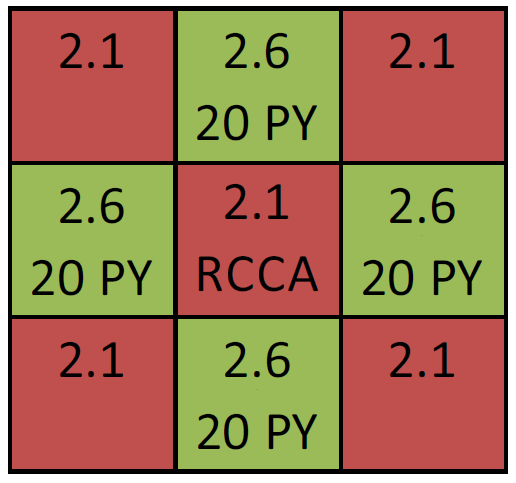
\includegraphics[width=\textwidth]{p4a_layout.png}
    \end{column}
    \begin{column}{0.22\textwidth}
        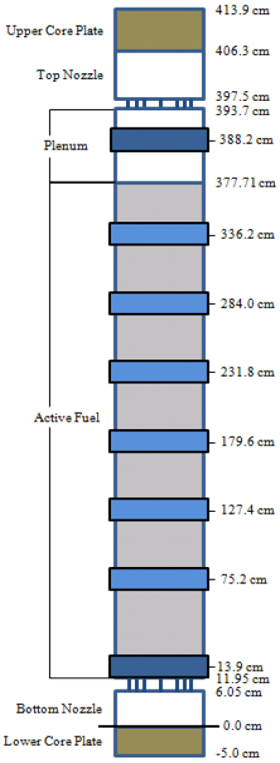
\includegraphics[width=\textwidth]{wb_3d_assembly.png}
\end{column}
\end{columns}
    
\end{frame}

%%%%%%%%%%%%%%%%%%%%%%%%%%%%%%%%%%%%%%%%%%%%%%%%%%%%%%%%%%%%%%%%%%%%%%%%%%%%%%%%%

\begin{frame}[t]{Test Procedures}
    
    \begin{itemize}
        \item Stuff
    \end{itemize}

\end{frame}

%%%%%%%%%%%%%%%%%%%%%%%%%%%%%%%%%%%%%%%%%%%%%%%%%%%%%%%%%%%%%%%%%%%%%%%%%%%%%%%%%

\begin{frame}[t]{Results}
    
    \begin{table}[h]
      \centering
      \resizebox{\textwidth}{!}{
        \begin{tabular}{|c|c|c|c|c|c|c|}\hline
          \multirow{2}{*}{Case} & k-eff & \multicolumn{2}{|c|}{Pin Power Differences} & \multicolumn{2}{|c|}{Iterations} & Runtime\\\cline{3-6}
          & Difference (pcm) & RMS & Max & 2D/1D & CMFD & (Core-Hours) \\\hline
          Reference        & -- & --     & --      & 12 & 364 & 8.59 \\\hline
          No Treatment     & -30 & 3.84\% & 21.81\% & 12 & 352 & 9.23 \\\hline
          Polynomial       & -8  & 1.03\% &  6.58\% & 12 & 360 & 9.50 \\\hline
          Sub-plane         & -7  & 1.13\% &  7.11\% & 12 & 409 & 9.26 \\\hline
          Sub-plane + 1D-CP & -2  & 0.54\% &  4.94\% & 12 & 364 & 9.45 \\\hline
        \end{tabular}
      }
    \end{table}
    \begin{itemize}
        \item Maximum error for all cases occurs in pins neighboring the partially rodded pin cell
    \end{itemize}
    
\end{frame}

%%%%%%%%%%%%%%%%%%%%%%%%%%%%%%%%%%%%%%%%%%%%%%%%%%%%%%%%%%%%%%%%%%%%%%%%%%%%%%%%%

\begin{frame}[t]{Differential Rod Worth Curve}
    
\begin{center}
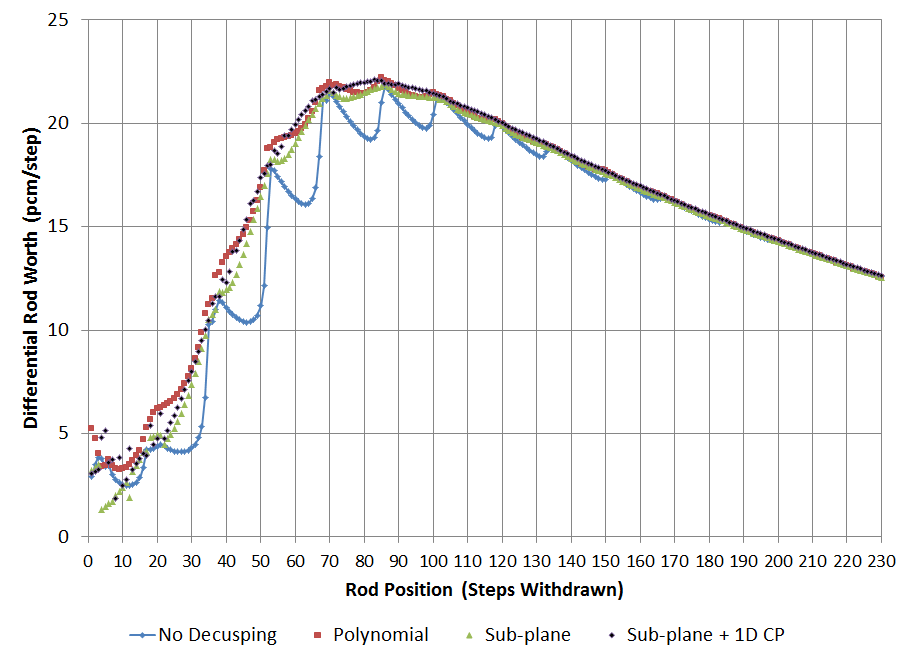
\includegraphics[width=0.8\textwidth]{differentialRodworth.png}
\end{center}
    
\end{frame}

%%%%%%%%%%%%%%%%%%%%%%%%%%%%%%%%%%%%%%%%%%%%%%%%%%%%%%%%%%%%%%%%%%%%%%%%%%%%%%%%%

\begin{frame}[t]{KENO-VI Comparisons}
    
    \begin{table}[h]
        \sisetup{separate-uncertainty=true,table-text-alignment=left,table-number-alignment=left}
        \resizebox{\textwidth}{!}{\begin{tabular}{l l 
                S[table-format=3.1,table-number-alignment=left] 
                S[table-format=1.3,table-number-alignment=left] 
                S[table-format=2.3,table-number-alignment=left]}\toprule
            \multirow{2}{*}{Cases} & \multirow{2}{*}{{Decusping Method}} & \multirow{2}{*}{{\keff{} 
                    Difference}} & 
            \multicolumn{2}{l}{{Pin Power Difference}} \\
            &  &  & {RMS} & {Max} \\\midrule
            \multirow{4}{*}{Average}       & None              &   -24.9 &  5.380\% & 25.902\% \\
            & Polynomial        &    34.8 &  1.502\% &  8.957\% \\
            & Subplane          &    34.6 &  0.984\% &  4.597\% \\
            & Subplane + CP     &    41.4 &  0.763\% &  3.386\% 
            \\\midrule
            \multirow{2}{*}{Worst -- 20\%} & None              & -176.0 & 14.709\% & 63.929\% \\
            & Polynomial        & 13.9   &  3.344\% & 25.373\% \\
            & Subplane          & 9.6    &  1.921\% &  9.900\% \\
            & Subplane + CP     & 45.9   &  1.324\% &  4.921\% \\
            \midrule
            Fully Withdrawn                & --                & 40.5   & 0.34\%   & 1.493\% \\
            \bottomrule
        \end{tabular}
    }
    \end{table}
\vfill
    
\end{frame}

%%%%%%%%%%%%%%%%%%%%%%%%%%%%%%%%%%%%%%%%%%%%%%%%%%%%%%%%%%%%%%%%%%%%%%%%%%%%%%%%%

\subsection{VERA Problem 5}
\begin{frame}[t]{Problem Description and Test Procedures}
    
    \begin{itemize}
      \item Bank D inserted to 257.9 cm, other banks all out
      \item 57 planes for tests and 58 for reference, 16 cores per plane
    \end{itemize}
    \begin{figure}[h]
      \centering
      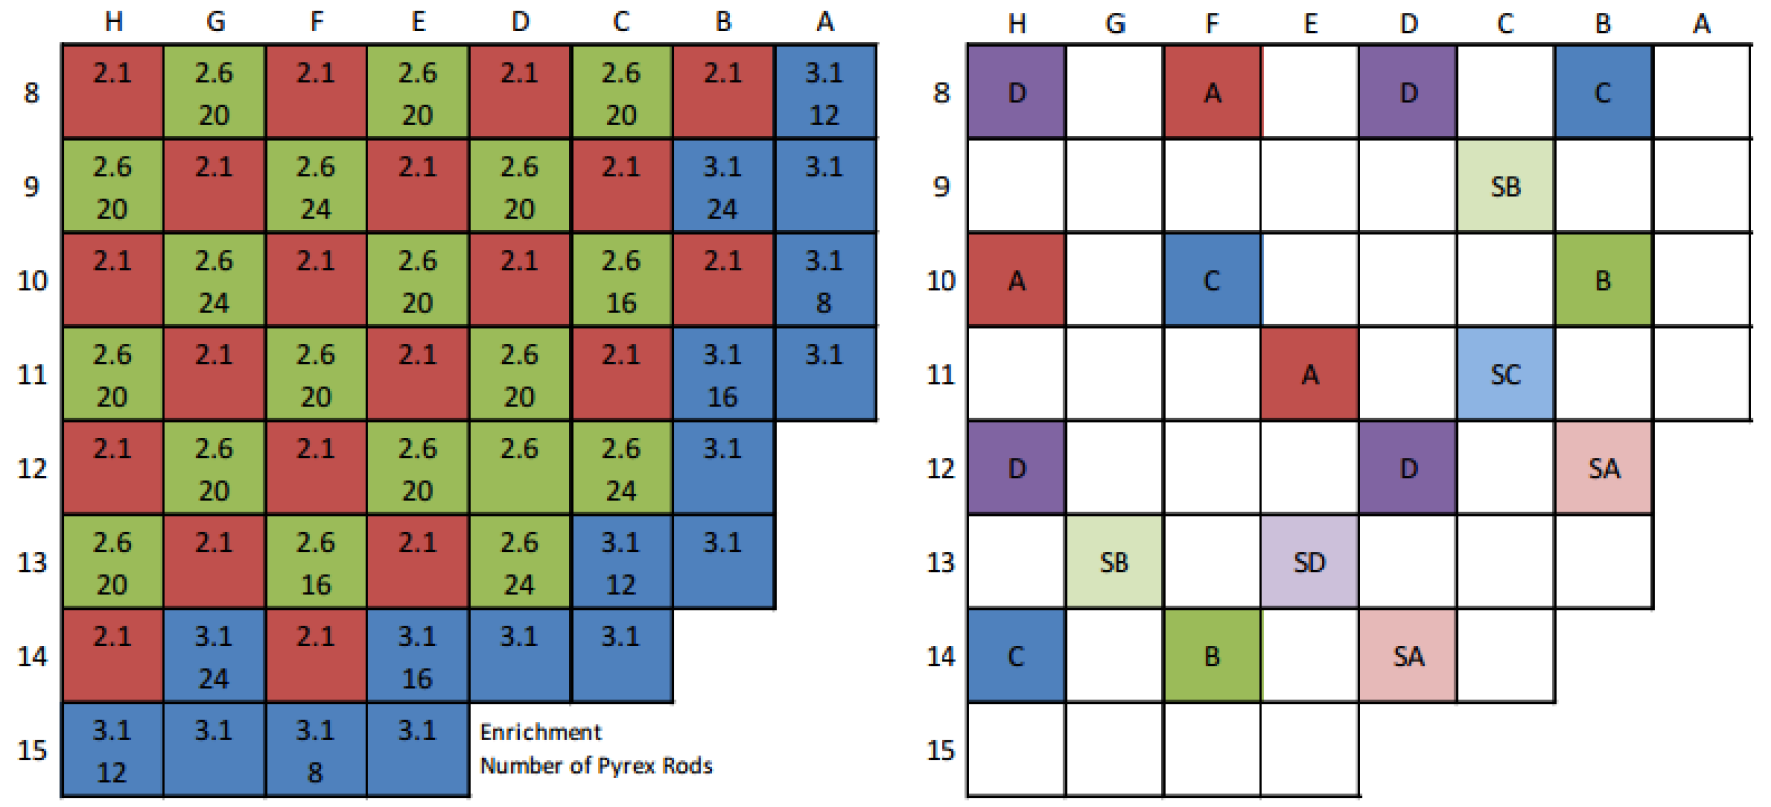
\includegraphics[width=0.9\textwidth]{WB1-cycle1-layout.png}
    \end{figure}
    
\end{frame}

%%%%%%%%%%%%%%%%%%%%%%%%%%%%%%%%%%%%%%%%%%%%%%%%%%%%%%%%%%%%%%%%%%%%%%%%%%%%%%%%%

\begin{frame}[t]{Problem 5 Results}
    
    \begin{table}[h]
      \centering
      \resizebox{\textwidth}{!}{
        \begin{tabular}{c c c c c c c}\toprule
        \multirow{2}{*}{Case} & \keff{} & \multicolumn{2}{c}{Pin Power Differences} & \multicolumn{2}{c}{Iterations} & Runtime\\
        & Difference (pcm) & RMS & Max & 2D/1D & CMFD & (Core-Hours) \\\midrule
        Reference        &  -- & --     & --      & 13 & 481 & 361.7 \\
        No Treatment     & -22 & 6.90\% & 30.55\% & 13 & 523 & 410.7 \\
        Polynomial       &  -5 & 1.15\% &  4.85\% & 13 & 463 & 373.7 \\
        Subplane         &  -5 & 2.09\% & 10.20\% & 13 & 499 & 399.0 \\
        Subplane + CP    &  -1 & 0.50\% &  2.74\% & 13 & 529 & 425.6 \\
        \bottomrule
    \end{tabular}
      }
    \end{table}
    \begin{itemize}
        \item Maximum error for each comparison occurs in pins neighboring the partially rodded pin cell
    \end{itemize}
    
\end{frame}

%%%%%%%%%%%%%%%%%%%%%%%%%%%%%%%%%%%%%%%%%%%%%%%%%%%%%%%%%%%%%%%%%%%%%%%%%%%%%%%%

\subsection{2D C5G7}
\begin{frame}[t]{Problem Description}
 
\begin{columns}
\begin{column}{0.6\textwidth}
\vspace{-0.25in}
\begin{center}
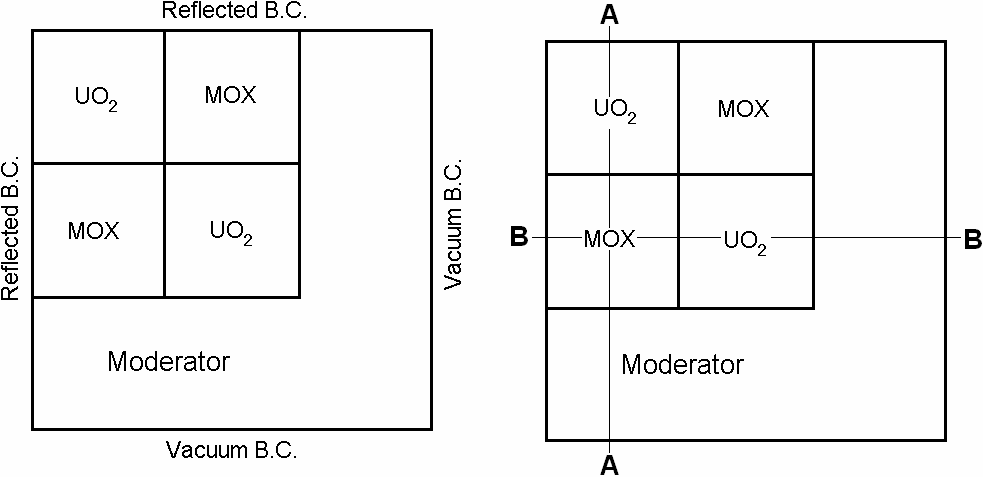
\includegraphics[width=\columnwidth]{c5g7-core-radial.png}

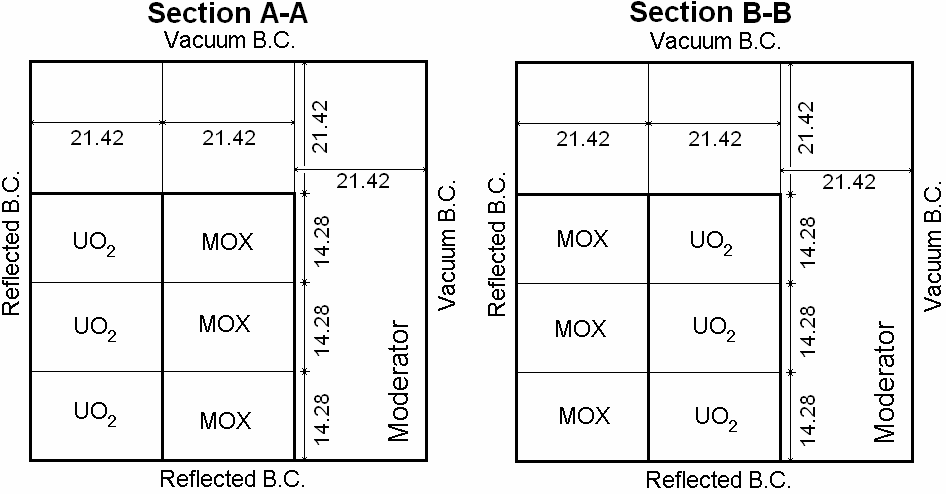
\includegraphics[width=\columnwidth]{c5g7-core-axial.png}
\end{center}
\end{column}
\begin{column}{0.4\textwidth}
    \begin{center}
    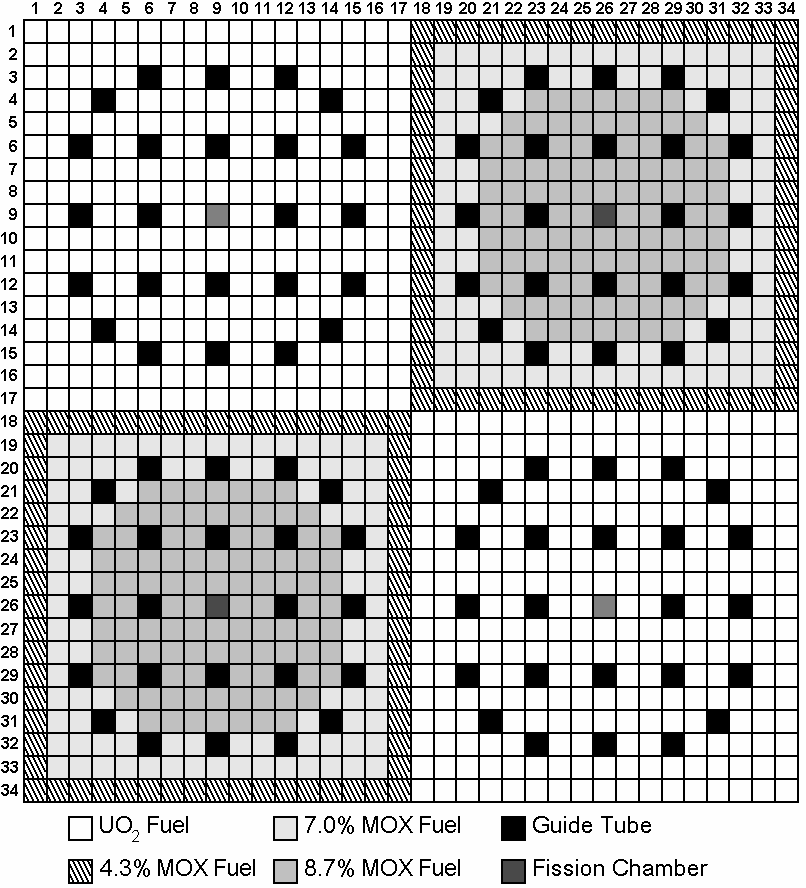
\includegraphics[width=\columnwidth]{c5g7-assemblies-radial.png}
\end{center}
\end{column}
\end{columns}
    
\end{frame}

%%%%%%%%%%%%%%%%%%%%%%%%%%%%%%%%%%%%%%%%%%%%%%%%%%%%%%%%%%%%%%%%%%%%%%%%%%%%%%%%

\begin{frame}[t]{Test Procedure}
    
    \begin{itemize}
        \item Explain
    \end{itemize}
    
\end{frame}

%%%%%%%%%%%%%%%%%%%%%%%%%%%%%%%%%%%%%%%%%%%%%%%%%%%%%%%%%%%%%%%%%%%%%%%%%%%%%%%%

\begin{frame}[t]{2D Core Results}

\begin{table}[h]
    \resizebox{\textwidth}{!}{
        \begin{tabular}{l l l l l l l l l l l l l l}
            \toprule
            Rod & Reference & \multicolumn{3}{c}{Subray-0} & \multicolumn{3}{c}{Subray-1} & \multicolumn{3}{c}{Subray-2} & \multicolumn{3}{c}{Subray-3} \\
            Position & \keff{} & \keff{} & \multicolumn{2}{l}{Pin Powers} & \keff{} & \multicolumn{2}{l}{Pin Powers} & \keff{} & \multicolumn{2}{l}{Pin Powers} & \keff{} & \multicolumn{2}{l}{Pin Powers} \\
            &  &  & RMS & Max &  & RMS & Max &  & RMS & Max &  & RMS & Max \\
            \midrule
            1* & 1.06839 & -15  & 0.10\% & 0.29\% & -15  & 0.10\% & 0.29\% & -15  & 0.10\% & 0.29\% & -15  & 0.10\% & 0.29\% \\
            2 & 1.07746 & -33  & 0.22\% & 0.67\% & -34  & 0.22\% & 0.68\% & -34  & 0.22\% & 0.67\% & -34  & 0.22\% & 0.67\% \\
            3 & 1.08777 & -53  & 0.32\% & 1.03\% & -56  & 0.34\% & 1.07\% & -55  & 0.34\% & 1.06\% & -55  & 0.34\% & 1.06\% \\
            4 & 1.09919 & -72  & 0.41\% & 1.34\% & -78  & 0.45\% & 1.45\% & -78  & 0.45\% & 1.44\% & -78  & 0.45\% & 1.44\% \\
            5 & 1.11160 & -89  & 0.46\% & 1.53\% & -99  & 0.51\% & 1.69\% & -98  & 0.50\% & 1.66\% & -98  & 0.50\% & 1.66\% \\
            6 & 1.12495 & -102 & 0.49\% & 1.66\% & -115 & 0.55\% & 1.83\% & -115 & 0.54\% & 1.82\% & -115 & 0.54\% & 1.81\% \\
            7 & 1.13925 & -112 & 0.49\% & 1.70\% & -127 & 0.55\% & 1.88\% & -126 & 0.55\% & 1.87\% & -126 & 0.55\% & 1.86\% \\
            8 & 1.15469 & -117 & 0.47\% & 1.65\% & -133 & 0.53\% & 1.83\% & -132 & 0.53\% & 1.81\% & -132 & 0.52\% & 1.81\% \\
            9* & 1.17190 & -117 & 0.43\% & 1.50\% & -127 & 0.46\% & 1.61\% & -126 & 0.46\% & 1.60\% & -126 & 0.46\% & 1.60\% \\
            \midrule
            Average & -- & 79 & 0.38\% & 1.26\% & 87 & 0.41\% & 1.37\% & 87 & 0.41\% & 1.36\% & 87 & 0.41\% & 1.36\% \\
            \bottomrule
        \end{tabular}
    }
\end{table}

\end{frame}

%%%%%%%%%%%%%%%%%%%%%%%%%%%%%%%%%%%%%%%%%%%%%%%%%%%%%%%%%%%%%%%%%%%%%%%%%%%%%%%%

\begin{frame}[t]{2D Core Results}

\begin{table}
    \centering
    \resizebox{\textwidth}{!}{
        \begin{tabular}{l l l l l l S[table-format=2.2,table-number-alignment=left] S[table-format=2.2,table-number-alignment=left] l l l l l l}
            \toprule
            Rod & Reference & \multicolumn{3}{c}{Subray-0} & \multicolumn{3}{c}{{None}} & \multicolumn{3}{c}{Subplane} & \multicolumn{3}{c}{Subplane + CP} \\
            Position & \keff{} & \keff{} & \multicolumn{2}{l}{Pin Powers} & {\keff{}} & \multicolumn{2}{l}{{Pin Powers}} & \keff{} & \multicolumn{2}{l}{Pin Powers} & \keff{} & \multicolumn{2}{l}{Pin Powers} \\
            &  &  & RMS & Max &  & {RMS} & {Max} &  & RMS & Max &  & RMS & Max \\
            \midrule
            1* & 1.06839 & -15  & 0.10\% & 0.29\% & -286  & 1.73 \% & 4.47 \% & -87  & 0.52\% & 1.35\% & -169 & 0.99\% & 2.46\% \\
            2  & 1.07746 & -33  & 0.22\% & 0.67\% & -811  & 4.75 \% & 12.70\% & -198 & 1.13\% & 3.06\% & -174 & 0.97\% & 2.57\% \\
            3  & 1.08777 & -53  & 0.32\% & 1.03\% & -1369 & 7.71 \% & 21.30\% & -290 & 1.56\% & 4.42\% & -181 & 0.97\% & 2.70\% \\
            4  & 1.09919 & -72  & 0.41\% & 1.34\% & -1918 & 10.33\% & 29.42\% & -360 & 1.83\% & 5.35\% & -185 & 0.94\% & 2.75\% \\
            5  & 1.11160 & -89  & 0.46\% & 1.53\% & -2400 & 12.25\% & 36.00\% & -405 & 1.93\% & 5.84\% & -184 & 0.88\% & 2.68\% \\
            6  & 1.12495 & -102 & 0.49\% & 1.66\% & -2738 & 13.12\% & 39.83\% & -424 & 1.89\% & 5.89\% & -174 & 0.78\% & 2.47\% \\
            7  & 1.13925 & -112 & 0.49\% & 1.70\% & -2820 & 12.55\% & 39.38\% & -416 & 1.72\% & 5.52\% & -155 & 0.65\% & 2.11\% \\
            8  & 1.15469 & -117 & 0.47\% & 1.65\% & -2478 & 10.08\% & 32.80\% & -377 & 1.44\% & 4.76\% & -124 & 0.48\% & 1.62\% \\
            9* & 1.17190 & -117 & 0.43\% & 1.50\% & -1461 & 5.31 \% & 18.00\% & -300 & 1.06\% & 3.60\% & -80  & 0.29\% & 1.00\% \\
            \midrule
            Average & -- & 79 & 0.38\% & 1.26\% & 1809 & 8.65\% & 25.99\% & 317 & 1.45\% & 4.42\% & 158 & 0.77\% & 2.26\% \\
            \bottomrule
        \end{tabular}
    }
\end{table}

\end{frame}

%%%%%%%%%%%%%%%%%%%%%%%%%%%%%%%%%%%%%%%%%%%%%%%%%%%%%%%%%%%%%%%%%%%%%%%%%%%%%%%%

\begin{frame}[t]{2D Core Performance}

\begin{columns}
\begin{column}{0.4\textwidth}
\begin{table}[h]
    \resizebox{\columnwidth}{!}{\begin{tabular}{l l l }\toprule
        Method & Long Rays per Plane & Increase \\\midrule
        Reference & 88440 & -- \\
        Subray-0 & 107400 & 21\% \\
        Subray-1 & 111792 & 26\% \\
        Subray-2 & 115264 & 30\% \\
        Subray-3 & 117920 & 33\% \\
        \bottomrule
    \end{tabular}
    }
\end{table}
\vfill
\end{column}

\begin{column}{0.6\textwidth}
\begin{table}[h]
    \resizebox{\columnwidth}{!}{\begin{tabular}{l l l l}\toprule
        Method & Iterations & Runtime (s) & Speedup \\\midrule
        Reference     & 25.7 & 1107 & --  \\
        None          & 25.8 & 739 & 1.50 \\ 
        Subplane      & 26.7 & 725 & 1.53 \\ 
        Subplane + CP & 26.9 & 695 & 1.61 \\
        Subray-0      & 26.4 & 861 & 1.29 \\ 
        Subray-1      & 25.9 & 881 & 1.26 \\ 
        Subray-2      & 26.1 & 920 & 1.21 \\ 
        Subray-3      & 26.1 & 938 & 1.18 \\ 
        \bottomrule
    \end{tabular}
}
\end{table}
\vfill
\end{column}
\end{columns}

\end{frame}

%%%%%%%%%%%%%%%%%%%%%%%%%%%%%%%%%%%%%%%%%%%%%%%%%%%%%%%%%%%%%%%%%%%%%%%%%%%%%%%%

\subsection{3D C5G7}
\begin{frame}[t]{Problem and Procedure Description}
    
    \begin{itemize}
        \item Stuff
    \end{itemize}

\end{frame}

%%%%%%%%%%%%%%%%%%%%%%%%%%%%%%%%%%%%%%%%%%%%%%%%%%%%%%%%%%%%%%%%%%%%%%%%%%%%%%%%

\begin{frame}[t]{3D Assembly Results}

\begin{table}[h]
    \resizebox{!}{0.25\textwidth}{\begin{tabular}{l l l l S[table-format=2.2,table-number-alignment=left]}\toprule
        \multirow{2}{*}{Case} & \multirow{2}{*}{Method} & \keff{} & \multicolumn{2}{l}{{Pin Powers}} \\
        &  & Diff. & RMS & {Max} \\\midrule
        \multirow{7}{*}{Average} & None        & 2193 & 6.05\% & 10.95\% \\
        & Subplane    & 222  & 0.88\% &  1.64\% \\
        & Subplane+CP & 114  & 0.45\% &  0.84\% \\
        & Subray-0    & 52   & 0.25\% &  0.54\% \\
        & Subray-1    & 56   & 0.25\% &  0.55\% \\
        & Subray-2    & 56   & 0.25\% &  0.54\% \\
        & Subray-3    & 56   & 0.25\% &  0.54\% \\
        \midrule
        \multirow{7}{*}{Position 8} & None          & -91 & 2.88\% & 4.19\% \\
        & Subplane      & -319  & 1.51\% & 2.66\% \\
        & Subplane + CP & -106 & 0.52\% & 0.89\% \\
        & Subray-0      & -104 & 0.53\% & 0.94\% \\
        & Subray-1      & -104 & 0.52\% & 0.94\% \\
        & Subray-2      & -105 & 0.53\% & 0.98\% \\
        & Subray-3      & -105 & 0.53\% & 0.98\% \\
        \bottomrule
    \end{tabular}
}
\end{table}

\end{frame}

%%%%%%%%%%%%%%%%%%%%%%%%%%%%%%%%%%%%%%%%%%%%%%%%%%%%%%%%%%%%%%%%%%%%%%%%%%%%%%%%

\begin{frame}[t]{3D Assembly Results}
    
    Plot of max power differences by rod position
    
\end{frame}

%%%%%%%%%%%%%%%%%%%%%%%%%%%%%%%%%%%%%%%%%%%%%%%%%%%%%%%%%%%%%%%%%%%%%%%%%%%%%%%%

\begin{frame}[t]{3D Assembly Performance}

\begin{columns}
\begin{column}{0.4\textwidth}
\begin{table}[h]
    \resizebox{\columnwidth}{!}{\begin{tabular}{l l l}\toprule
        Method & Long Rays per Plane & Increase \\\midrule
        Reference & 29480 & -- \\
        Subray-0 & 48440 & 64\% \\
        Subray-1 & 52832 & 79\% \\
        Subray-2 & 56304 & 91\% \\
        Subray-3 & 58960 & 100\% \\
        \bottomrule
    \end{tabular}
}
\end{table}
\vfill
\end{column}

\begin{column}{0.6\textwidth}
\begin{table}[h]
    \resizebox{\columnwidth}{!}{\begin{tabular}{l l l l}\toprule
        Method & Iterations & Runtime (s) & Speedup \\\midrule
        Reference     & 27.5 & 490 & --   \\
        None          & 27.8 & 361 & 1.36 \\
        Subplane      & 27.5 & 374 & 1.32 \\
        Subplane + CP & 27.2 & 353 & 1.39 \\
        Subray-0      & 27.6 & 444 & 1.11 \\
        Subray-1      & 28.7 & 464 & 1.07 \\
        Subray-2      & 28.8 & 475 & 1.04 \\
        Subray-3      & 28.8 & 478 & 1.03 \\
        \bottomrule
    \end{tabular}
}
\end{table}
\vfill
\end{column}
\end{columns}

\end{frame}

%%%%%%%%%%%%%%%%%%%%%%%%%%%%%%%%%%%%%%%%%%%%%%%%%%%%%%%%%%%%%%%%%%%%%%%%%%%%%%%%

\begin{frame}[t]{3D Core Results}

\begin{table}[h]
    \resizebox{!}{0.25\textwidth}{\begin{tabular}{l l l S[table-format=2.2,table-number-alignment=left] S[table-format=2.2,table-number-alignment=left]}\toprule
        \multirow{2}{*}{Case} & \multirow{2}{*}{Method} & \keff{} & \multicolumn{2}{l}{{Pin Powers}} \\
        & & Diff. & {RMS} & {Max} \\\midrule
        \multirow{7}{*}{Average} & None        & 21 & 6.62\% & 29.30\% \\
        & Subplane    & 21 & 0.69\% & 3.47 \% \\
        & Subplane+CP & 21 & 0.34\% & 1.69 \% \\
        & Subray-0    & 21 & 0.20\% & 1.06 \% \\
        & Subray-1    & 25 & 0.20\% & 1.14 \% \\
        & Subray-2    & 25 & 0.20\% & 1.11 \% \\
        & Subray-3    & 21 & 0.20\% & 1.11 \% \\
        \midrule
        \multirow{7}{*}{Position 16} & None          & -1730 & 12.62\% & 55.69\% \\
        & Subplane      & -183 & 1.08\% & 5.61\% \\
        & Subplane + CP & -76 & 0.45\% & 2.38\% \\
        & Subray-0      & -46 & 0.30\% & 1.76\% \\
        & Subray-1      & -54 & 0.35\% & 2.01\% \\
        & Subray-2      & -53 & 0.34\% & 1.97\% \\
        & Subray-3      & -53 & 0.34\% & 1.96\% \\
        \bottomrule
    \end{tabular}
}
\end{table}

\end{frame}

%%%%%%%%%%%%%%%%%%%%%%%%%%%%%%%%%%%%%%%%%%%%%%%%%%%%%%%%%%%%%%%%%%%%%%%%%%%%%%%%

\begin{frame}[t]{3D Core Results}

Plot of max power differences by rod position

\end{frame}

%%%%%%%%%%%%%%%%%%%%%%%%%%%%%%%%%%%%%%%%%%%%%%%%%%%%%%%%%%%%%%%%%%%%%%%%%%%%%%%%

\begin{frame}[t]{3D Core Performance}

\begin{table}[h]
    \begin{tabular}{l l l l}\toprule
        Method & Iterations & Runtime (s) & Speedup \\\midrule
        Reference     & 27.8 & 3256 & -- \\
        None          & 28.2 & 2581 & 1.25 \\
        Subplane      & 29.1 & 2454 & 1.32 \\
        Subplane + CP & 28.9 & 2454 & 1.32 \\
        Subray-0      & 28.8 & 2851 & 1.13 \\
        Subray-1      & 28.9 & 2920 & 1.11 \\
        Subray-2      & 29.1 & 2963 & 1.09 \\
        Subray-3      & 29.2 & 3009 & 1.08 \\
        \bottomrule
    \end{tabular}
\end{table}
\vfill

\end{frame}